\documentclass{beamer}
\usepackage[russian]{babel}
\usetheme{metropolis}

\usepackage{amsthm}
\setbeamertemplate{theorems}[numbered]

\setbeamercolor{block title}{use=structure,fg=white,bg=gray!75!black}
\setbeamercolor{block body}{use=structure,fg=black,bg=gray!20!white}

\usepackage[T2A]{fontenc}
\usepackage[utf8]{inputenc}

\usepackage{hyphenat}
\usepackage{amsmath}
\usepackage{graphicx}

\AtBeginEnvironment{proof}{\renewcommand{\qedsymbol}{}}{}{}

\title{
Микроэкономика-I
}
\author{
Павел Андреянов, PhD
}

\begin{document}

\maketitle

\begin{frame}{План лекции}
\begin{itemize}
  \item Часть 1. Разбор контрольной.
  \item Часть 2. Парето оптимальность и (общее) равновесие Вальраса в экономике обмена. Равновесие с трансфертами.
\end{itemize}
\end{frame}

\section{Экономика обмена}

\begin{frame}{Экономика обмена}
\alert{Экономика обмена} - это когда нет производства. Ресурсы и товары изначально распределены между экономическими агентами и затем \alert{торгуются на конкурентном рынке или меняются при помощи бартера}.
\end{frame}

\begin{frame}{Пример}
У крестьянина $a$ есть яблоневый сад, он приносит ему 100 яблок каждый год. У крестьянина $b$ есть куры которые несут 150 яиц в год. 

Другими словами, \alert{начальные запасы} крестьянина $a$ описываются вектором $\vec w_a = (100,0)$ а крестьянина $b$ вектором $\vec w_b = (0,150)$. 

\alert{Общие запасы} описываются вектором $\vec w = (100,150)$.


\end{frame}

\begin{frame}{Пример}

Другими словами, \alert{начальные запасы} крестьянина $a$ описываются вектором $\vec w_a = (100,0)$ а крестьянина $b$ вектором $\vec w_b = (0,150)$. \alert{Общие запасы} описываются вектором $\vec w = (100,150)$.

\begin{itemize}
  \item \alert{бартер}: крестьяне обменяли 50 яблок на 50 куриных яиц
  \item \alert{торговля}: крестьянин $a$ решил потребить $\vec x_a = (50, 50)$, а крестьянин $b$ решил потребить $\vec x_b = (50, 100)$ яблок. 
\end{itemize}

В сценарии с торговлей, мы представляем себе, что крестьяне сначала продают все свои запасы на рынке, получают деньги, а потом решают задачу максимизации полезности. 

Цены устанавливает некая беневолентная сущность.

\end{frame}

\begin{frame}{Формально}

Мы хотим ответить на следующие вопросы: какие состояния экономики возможны в результате бартера? какие состояния экономики возможны в результате торговли.

Попробуем эту идею формализовать...

Пусть у нас есть $I = \{a,b,c, \ldots \}$ агентов и $K = \{1,2,3, \ldots \}$ товаров.
\end{frame}

\section{Допустимые состояния}
\begin{frame}{Допустимые состояния}

\alert{Допустимым состоянием} экономики обмена называется набор координат потреблений
$$ \vec x = \{ \vec x_a, \vec x_b, \vec x_c, \ldots \},$$
такой, что потребления неотрицательные
$$\forall i \in I, \quad k \in K, \quad 0 \leqslant x_{ik}$$
а сумма (по агентам $i \in I$) потреблений 
$$\forall k \in K, \quad \sum_{i \in I} x_{ik} = \sum_{i \in I} w_{ik}$$
совпадает с общими запасами для каждого товара (по отдельности).
\end{frame}

\begin{frame}{Формально}
Рассмотрим случай, когда $\dim I = 2, \dim K = 2$. В таком случае, допустимые состояния описываются четырьмя координатами:
$$ x_{a1}, \ x_{a2}, \ x_{b1}, \ x_{b2},$$
причем они связаны соотношениями
$$ x_{b1} = w_{a1} + w_{b1} - x_{a1}, \quad x_{b2} = w_{a2} + w_{b2} - x_{a2}$$
то есть \alert{степеней свободы} у допустимого состояния всего две, например ими могли бы быть координаты потребления первого агента: $x_{a1}, x_{a2}$. 

Действительном, координаты потребления второго агента выражаются через них и запасы (которые известны и постоянны).
\end{frame}

\section{Ящик Эджворта}

\begin{frame}{Фрэнсис Эджуорт}
\begin{columns}
\begin{column}{0.5\textwidth}
   \alert{Фрэнсис Эджуорт} (Francis Edgeworth) английский экономист второй половины 19 века. 
   
  Был сторонником идеи прогрессивного налогообложения, мотивируя его убывающей предельной полезностью доходов. В честь него названы ящик Эджуорта и налоговый парадокс Эджуорта.
\end{column}
\begin{column}{0.5\textwidth}  %%<--- here
    \begin{center}
     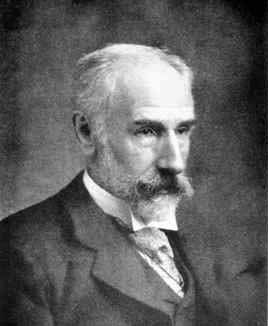
\includegraphics[width=1\textwidth]{Edgeworth}
     \end{center}
\end{column}
\end{columns}
\end{frame}

\begin{frame}{Ящик Эджворта}
Пространство допустимых состояний описывается прямоугольником в $\mathbb{R}^2$, высота и ширина которого равны $\vec w = (w_1,w_2)$ соответственно. Этот прямоугольник называется \alert{ящиком Эджворта}, в честь еще одного экономиста.

На той же картинке мы можем изобразить предпочтения каждого агента. Для этого надо выбрать того агента, чьи координаты будут расположены нормально, а координаты второго агента будут перевернуты. 

По умолчанию мы переворачиваем второго агента ($b$).
\end{frame}

\begin{frame}{Ящик Эджворта}
Гениальность конструкции в том, что все точки внутри ящика представляют собой все допустимые состояния экономики.
    \begin{center}
     \includegraphics[width=.8\textwidth]{edge}
     \end{center}
\end{frame}

\section{Парето оптимальность}

\begin{frame}{Вильфредо Парето}
\begin{columns}
\begin{column}{0.5\textwidth}
   \alert{Вильфредо Парето} (Vilfredo Pareto) итальянский математик и экономист второй половины 19 века. 
   
  Он разработал теории, названные впоследствии его именем: статистическое Парето-распределение и Парето-оптимум, широко используемые в экономической теории и иных научных дисциплинах.
\end{column}
\begin{column}{0.5\textwidth}  %%<--- here
    \begin{center}
     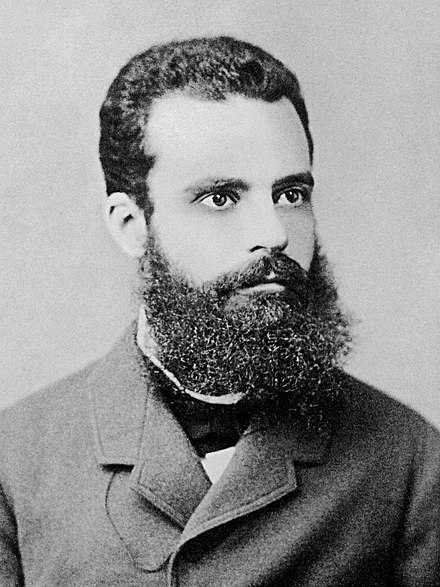
\includegraphics[width=1\textwidth]{Pareto}
     \end{center}
\end{column}
\end{columns}
\end{frame}


\begin{frame}{Парето оптимальность}
Далее, мы хотим выбрать те допустимые состояния экономики из которых нельзя выйти при помощи бартера, а значит они будут потенциальными "равновесиями" в бартерной системе.

Допустимое состояние $x$ это \alert{(слабый) Парето оптимум}, если не существует другого допустимого состояния, которое делает всем агентам (сильно) лучше.
	
Формально, это можно определить как $$E \cap L^a_{++}(x) \cap L^b_{++}(x) = \emptyset,$$ где $E$ это сам ящик Эджворта.

Все такие точки называются \alert{Парето границей} или \alert{Парето фронтом}.
\end{frame}


\begin{frame}{Парето оптимальность}
Какие из трех точек $x^{\ast}, \hat x, \tilde x$ являются Парето оптимальными?
  \begin{center}
     \includegraphics[width=.8\textwidth]{edge2}
     \end{center}
\end{frame}

\begin{frame}{Парето оптимальность}

Допустимое состояние это \alert{(сильный) Парето оптимум}, если не существует другого допустимого состояния, которое делает всем агентам (слабо) лучше, но хотя бы одному агенту – сильно.

Формально, это можно определить как $$E \cap (L^a_{++}(x) \cap L^b_{+}(x)) \cup (L^a_{+}(x) \cap L^b_{++}(x))= \emptyset.$$

Пример слабого но не сильного ПО легко построить при помощи толстой кривых безразличия.

\end{frame}

\begin{frame}{Парето оптимальность}

Сильные ПО это подмножество слабых ПО, но мы почти никогда не будем различать их между собой.

Дело в том, что для подавляющего числа задач они вообще совпадают. Чаще всего это просто точки касания кривых безразличия.

Но есть и исключения (все они связаны с границей ящика).
\end{frame}

\begin{frame}{Экзотический пример 1}
Пусть в ящике Эджворта первая полезность квазилинейная, а вторая КД.

\begin{center}
     \includegraphics[width=.8\textwidth]{edge3}
     \end{center}

\end{frame}

\begin{frame}{Экзотический пример 2}
Пусть в ящике Эджворта первая полезность линейная, а вторая Леонтьев.

\begin{center}
     \includegraphics[width=.8\textwidth]{edge4}
     \end{center}

\end{frame}

\section{Примеры у доски}

\begin{frame}{Примеры у доски}
Опять пусть есть два агента с запасами (1,2) и (1,1).
\begin{itemize}
  \item $U_a(x,y) = U_b(x,y) = \alpha \log x + \log y$\
  \item $U_a(x,y) = \log x + y, \quad U_b(x,y) = \alpha \log x + \log y $
  \item $U_a(x,y) = \min(x,y), \quad U_b(x,y) = \alpha \log x + \log y $
  \item $U_a(x,y) = \sqrt{x}+ \sqrt{y}, \quad U_b(x,y) = \alpha x + y $
\end{itemize}
Нарисуйте (слабую) Парето границу. Какие точки на границе не могут быть результатом добровольного бартера, подразумевая что агенты не будут меняться себе в ущерб?
\end{frame}

\section{Равновесие Вальраса}

\begin{frame}{Леон Вальрас}
\begin{columns}
\begin{column}{0.5\textwidth}
   \alert{Леон Вальрас} (Leon Walras) французский экономист второй половины 19 века. 
   
Лидер Лозаннской школы маржинализма. 

Основатель теории общего экономического равновесия.
\end{column}
\begin{column}{0.5\textwidth}  %%<--- here
    \begin{center}
     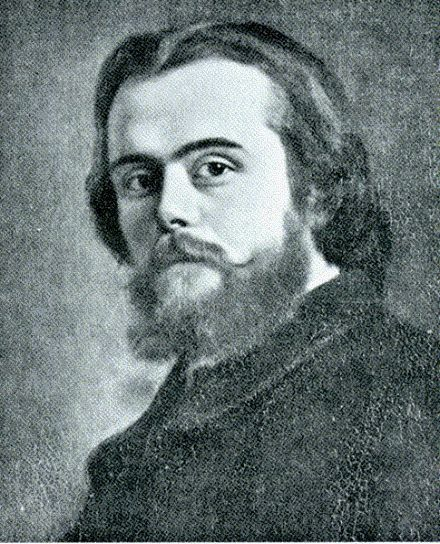
\includegraphics[width=1\textwidth]{Walras}
     \end{center}
\end{column}
\end{columns}
\end{frame}

\begin{frame}{Равновесие Вальраса}
\alert{Равновесием Вальраса} экономики обмена называется допустимое состояние $\vec x$ и вектор цен $\vec p$, такие, что каждый агент достигает максимума полезности по бюджетному ограничению с бюджетом, равным доходу от продажи своих начальных запасов.
$$ \forall i \in I, \quad \vec x_i \in arg \max U_i(\ast) \quad s.t. \quad \vec p \cdot \vec x_i \leqslant \vec p \cdot \vec w_i$$

Другими словами РВ - это модель состояния торговой площадки. Существование РВ - неочевидное утверждение.
\end{frame}

\begin{frame}{Как устроена площадка}

Денег изначально у агентов нет, а есть только запасы.

\begin{itemize}
  \item На табло высвечивается некоторый вектор цен $\vec p$.
  \item Агенты меняют все запасы на деньги, теперь у агентов только деньги, а товаров нет.
  \item Далее, агент заказывает себе товары максимизируя полезность при бюджетном ограничении
  \item Снова у агентов есть товары но нет денег (вернее, у них талоны от заказанных товаров но не сами товары)
\end{itemize}

Если не возникло дефицита и все заказы были успешно выполнены, то это и есть равновесие. Наша задача понять при каких ценах $\vec p$ это верно.

\end{frame}

\section{Закон Вальраса}
\begin{frame}{Закон Вальраса}
Напомним, что при \alert{локальной ненасыщаемости} полезностей, агенты полностью тратят все свои деньги: 
$$ \forall i \in I, \quad \vec p \cdot \vec x_i = \vec p \cdot \vec w_i,$$
это называется \alert{Законом Вальраса}. 

Формально это не является частью определения РВ, но практически моментально вытекает из него. 
\end{frame}

\begin{frame}{Денежное Равенство}
Отсюда можно сделать вывод, что после окончания торгов у агентов не останется денег на руках, другими словами, выполнено \alert{денежное равенство}:
$$\quad \sum_{i \in I} \vec p \cdot \vec x_i = \sum_{i \in I} \vec p \cdot \vec w_i.$$
Действительно, справа стоят все деньги, полученные после продажи начальных запасов, а слева – все деньги, потраченные на покупку товаров.

Геометрически, это можно представить себе как \alert{ортогональность вектора цен $\vec p$ вектору $\vec x-\vec w$}.

\end{frame}

\section{РВ как система уравнений}

\begin{frame}{РВ как система уравнений}
Поиск Равновесия Вальраса можно представить себе как несколько групп уравнений.

\begin{itemize}
  \item товарные равенства, $K$ штук: что сумма товаров в каждой категории равны соответствующим общим запасам, т. е. допустимое состояние экономики;
  \item условия оптимальности, $K \cdot I$ штук: что каждый агент выбирает потребление оптимально, т. е. условия первого порядка;
  \item законы Вальраса, $I$ штук. Денежное равенство из них вытекает, поээтому мы его считать не будем.
\end{itemize}

\end{frame}

\begin{frame}{РВ как система уравнений}
Неизвестные тоже можно разбить на группы:

\begin{itemize}
  \item цены, их $K$ штук
  \item собственно потребления, их $K \cdot I$ штук
  \item множители Лагранжа, их $I$ штук
\end{itemize}

Казалось бы, у нас система из $I\cdot K + K + I$ уравнений и столько же неизвестных, но есть один подвох - система линейно зависима. 

\end{frame}

\begin{frame}{РВ как система уравнений}
Дело в том, что если выполнены все товарные равенства, то есть мы находимся в ящике Эджворта, и выполнены законы Вальраса для всех кроме одного агента, то \alert{последний закон Вальраса выполняется автоматически}. 

Если все кроме одного агента потратили все деньги, и товары перешли из одних руки в другие, то из этого алгебраически вытекает, что последний агент также потратил все свои деньги. 

\end{frame}

\begin{frame}{РВ как система уравнений}
То есть линейно независимых уравнений, на самом деле, $I\cdot K + K + I - 1$.

Получается, что уравнений больше, чем неизвестных?

\end{frame}

\begin{frame}{РВ как система уравнений}

На самом деле, неизвестных тоже $I\cdot K + K + I - 1$, ведь цены определены с точностью до константы, а значит цену одного из товаров (обычно последнего) можно приравнять к 1, без потери общности.

\end{frame}

\section{Связь ПО и РВ}
\begin{frame}{Связь ПО и РВ}
Легко видеть, что первый блок уравнений (товарные равенства) у РВ и ПО - одинаковый. Они просто фиксируют ящик Эджворта и точку начальных запасов в нем.

Второй блок уравнений (условия оптимальности), на самом деле, тоже совпадает в выпуклых задачах, потому что это условия касания кривых безразличия.

Наконец, третий блок (законы вальраса) это условие того, что бюджетная линия проходит сразу через две точки: начальные запасы и предполагаемое РВ.
\end{frame}

\begin{frame}{Связь ПО и РВ}
Получается, что РВ - выбирает на Парето-фронте (как правило) одну точку.
\begin{center}
     \includegraphics[width=.8\textwidth]{edge7}
     \end{center}
\end{frame}

\section{РВ против ПО}

\begin{frame}{РВ против ПО}
В чем разница между РВ и ПО?

\alert{В Равновесии Вальраса есть цены}, это главное. Происхождение этих цен нас не интересует, можно считать, что они написаны кем-то на гигантском табло. 

Каждый агент продает свои запасы по этим ценам и уже далее максимизирует полезность, покупая на эти деньги товары.

\end{frame}

\begin{frame}{РВ против ПО}
Возникает бюджетная линия, которая отделяет верхние Лебеговы множества агентов друг от друга в ящике Эджворта

\begin{center}
     \includegraphics[width=.9\textwidth]{edge5}
     \end{center}

\end{frame}

\begin{frame}{РВ против ПО}

\alert{В Парето оптимуме никаких цен нет}, соответственно бюджетных множеств тоже нет. 

В отличие о РВ, в ПО верхние Лебеговы множества не обязательно разделены линейно. 

Они могут быть разделены, например, параболой.

\end{frame}

\begin{frame}{РВ против ПО}
Поэтому верхние Лебеговы множества $L_{++}$ отделены друг от друга просто как нибудь.

\begin{center}
     \includegraphics[width=.9\textwidth]{edge6}
     \end{center}

\end{frame}

\begin{frame}{РВ против ПО}

Конечно, если экономика полностью выпуклая, то разделение всегда будет линейное, по Теореме о Разделяющей Гиперплоскости.

Но, вообще говоря, РВ это усиление ПО.

\alert{Первая Теорема Благосостояния}: любое РВ это слабое ПО.

Доказательство от противного...

\end{frame}

\begin{frame}{РВ против ПО}

Пусть точка $x$ является РВ с ценами $\vec p$ но не слабым ПО.

Тогда, по определению $L^a_{++}(x) \cap L_{++}^b(x) \cap E$ непусто. Получается, что есть некоторая другая точка $y$ которая
\begin{itemize}
  \item является допустимым состоянием экономики
  \item дает строго большую полезность обоим агентам
\end{itemize}
Поскольку точка $y$ лежит в ящике эджворта то она лежит либо над, либо под, либо в точности на бюджетной линии. Значит, ее точно мог бы купить один из двух агентов.

Но это противоречит оптимизации полезности в РВ.
\end{frame}

\section{РВ с трансфертами}

\begin{frame}{РВ с трансфертами}
\alert{Равновесием Вальраса с трансфертами} экономики обмена называется допустимое состояние $\vec x$ и вектор цен $\vec p$, такие, что каждый агент достигает максимума полезности по бюджетному ограничению, с бюджетом равным доходу от продажи своих начальных запасов \alert{плюс трансферты}.
$$ \forall i \in I, \quad \vec x_i \in arg \max U_i(\ast) \quad s.t. \quad \vec p \cdot \vec x_i \leqslant \vec p \cdot \vec w_i + T_i.$$
Очень важно, что \alert{трансферты суммируются в ноль} $\sum T_i = 0$, иначе сломается денежное равенство.

\end{frame}

\begin{frame}{РВ с трансфертами}
По сути, трансферты являются (скрытым) способом изменить начальные запасы и, как следствие, равновесие и цены. 
\begin{center}
     \includegraphics[width=.9\textwidth]{edge8}
     \end{center}
\end{frame}


\end{document}